% !TeX root = ./corona_contact_tracing.tex
% chktex-file 46
% !TeX spellcheck = en-GB
% !TeX encoding = utf8


\documentclass[]{article}

\RequirePackage{color,graphicx}
\usepackage{float}
\usepackage{longtable}
\usepackage{tabu}
\usepackage{pdfpages}
\usepackage{amsmath}
\usepackage{amsfonts}
\usepackage{amssymb}
\usepackage{mathtools}
\usepackage{csquotes}
\usepackage{cleveref}
\usepackage[american]{babel}
\usepackage[babel=true, protrusion=alltext-nott, final]{microtype}
\usepackage[nodayofweek]{datetime}
\usepackage[inline]{enumitem}
\usepackage{url}
\usepackage{todonotes}
\usepackage{biblatex}
\addbibresource{bibliography.bib}

%opening
\title{Corona Contact Tracing}
\author{Martin, Leonard, Thomas, Matthias}

\newcommand{\indexOfState}[1]{\texttt{indOfState}(#1)}
\DeclarePairedDelimiter\abs{\lvert}{\rvert}%
\DeclarePairedDelimiter\norm{\lVert}{\rVert}%

\setlength{\parskip}{1em}
\setlength{\parindent}{0cm}

\begin{document}

\maketitle

\begin{abstract}
	This technical report accompanies the implementation of the corona\_-contact\_tracing package found at \url{https://github.com/PellelNitram/corona_contact_tracing}.

	It extends an existing stochastic SIR simulation to generate data sets suitable to simulating the current corona pandemic.
	This simulation has full access to all agents' health status.
	To mirror a real world scenario the health status of agents is only partially observed through tests.

	Next we develop a graph convolutional approach to predict the health status of all agents in this simulation.
	It uses past contacts as well as observed health information to derive this prediction.
	It is able to deal with partial data such as missing locations and missing health status, as it is a probabilistic approach.
	
	Lastly, this prediction can be used to derive measures to reduce the diseases' spread.
	We propose to find a optimal trade of between removing the least amount of edges in said graph (e.g.\ through quarantine, social distancing, etc.) and limiting the spread of the disease.
	% Such trade of could be found with minimal cut algorithms.
	Opposed to classical non-pharmaceutical intervention methods such as contact tracing, our approach directly identifies the nodes with the greatest potential to accelerate the diseases' spread in the network.
	
	This technical report was created within the \#WirVsVirus Hackathon of the German government and is Work in Progress!
\end{abstract}


% !TeX root = ./corona_contact_tracing.tex
% chktex-file 46
% !TeX spellcheck = en-GB
% !TeX encoding = utf8

\section{Introduction}
The outbreak of the SARS-COV-2 virus and the associated COVID-19 illness sweeps rapidly across the world.
Some patients need ventilation support to survive and the exponential growth in infected persons quickly overwhelms any available medical resources.\\
Thus the identification of contact persons is of great importance to control the spread of the disease.
Some governments such as Singapurian use location trace data from mobile phone providers.
Other approaches are more user centric and build apps, which utilize GPS data of individuals.

It is known from past outbreaks and epidemilogic research that such contact tracing and non pharmaceutical interventions (NPI) like school cancellations are important tools. 
But both are not very directed interventions and do not reveal anything about the health state of the entire population.

The following section will first explain the mathematical foundations of our SIR model to generate realistic ground truth data.
Afterwards our novel graph-based approach to probabilistic health prediction of the entire population will be explained.
From location traces and some known infections it computes well educated guesses about the health state of the entire population.

In the outlook we sketch how this approach can be utilized to measure the effect of contact tracing and NPIs.
Furthermore, we propose to use mathematical optimization to compute very targeted NPIs (e.g.\ only cancellation of large events) and optimal placement of limited tests (e.g.\ prioritize potential super spreaders).
This controls the disease with minimal effects on daily life.

% !TeX root = ./corona_contact_tracing.tex
% chktex-file 46
% !TeX spellcheck = en-GB
% !TeX encoding = utf8

\section{Algorithm notes}

% !TeX root = ./corona_contact_tracing.tex
% chktex-file 46
% !TeX spellcheck = en-GB
% !TeX encoding = utf8

\subsection{SIR Model}
Our basic stochastic SIR model relies on the assumptions that every person in an environment can be modeled as a point value, which has a location (i.e.\ GPS coordinates) and an infection state. These states can be either \textit{susceptible} (S), \textit{infected} (I), \textit{recovered} (R) or in advanced models also \textit{under quarantine} (Q) or \textit{dead} (D). All individuals, here called agents, have a probability (here called diffusion rate $d$ to make a step per time step on a predefined grid. In the case, that some agents meet at the same location, disease spreading can occur. An infected agent spreads the disease with probability $\beta$ to all the agents in its close vicinity (same location on the grid). Furthermore recovery is covered by taking a recovery rate into account, i.e.\ a probability $\gamma$ to recover from the disease per time step. If an infected agent recovers from the disease, the state of the agent changes from \textit{infected} to \textit{recovered}, which is definite (no double infections). The process ends, when no infected agents are left.
\begin{center}
    Susceptibles $\overset{\beta}{\longrightarrow}$ Infected $\overset{\gamma}{\longrightarrow}$ Recovered.
\end{center}

An example of a early model state is shown in Figure~\ref{fig:1}
\begin{figure}[H]
    \centering
    \includegraphics[width=0.4\linewidth]{initial_setup.png}
    \caption{Early state of SIR model, blue dots = susceptibles, red dots = infected agents, green dots = Recovered agents}%
    \label{fig:1}
\end{figure}

In this case, 1000 agents were initialized on a 100 by 100 grid, where a certain amount of infected agents were introduced as a seed. Letting the agents perform random walks on the grid (maximally one step each time step with probability $d$), and letting the model converge, the results in figure~\ref{fig:2} can be observed.

\begin{figure}[H]
    \centering
    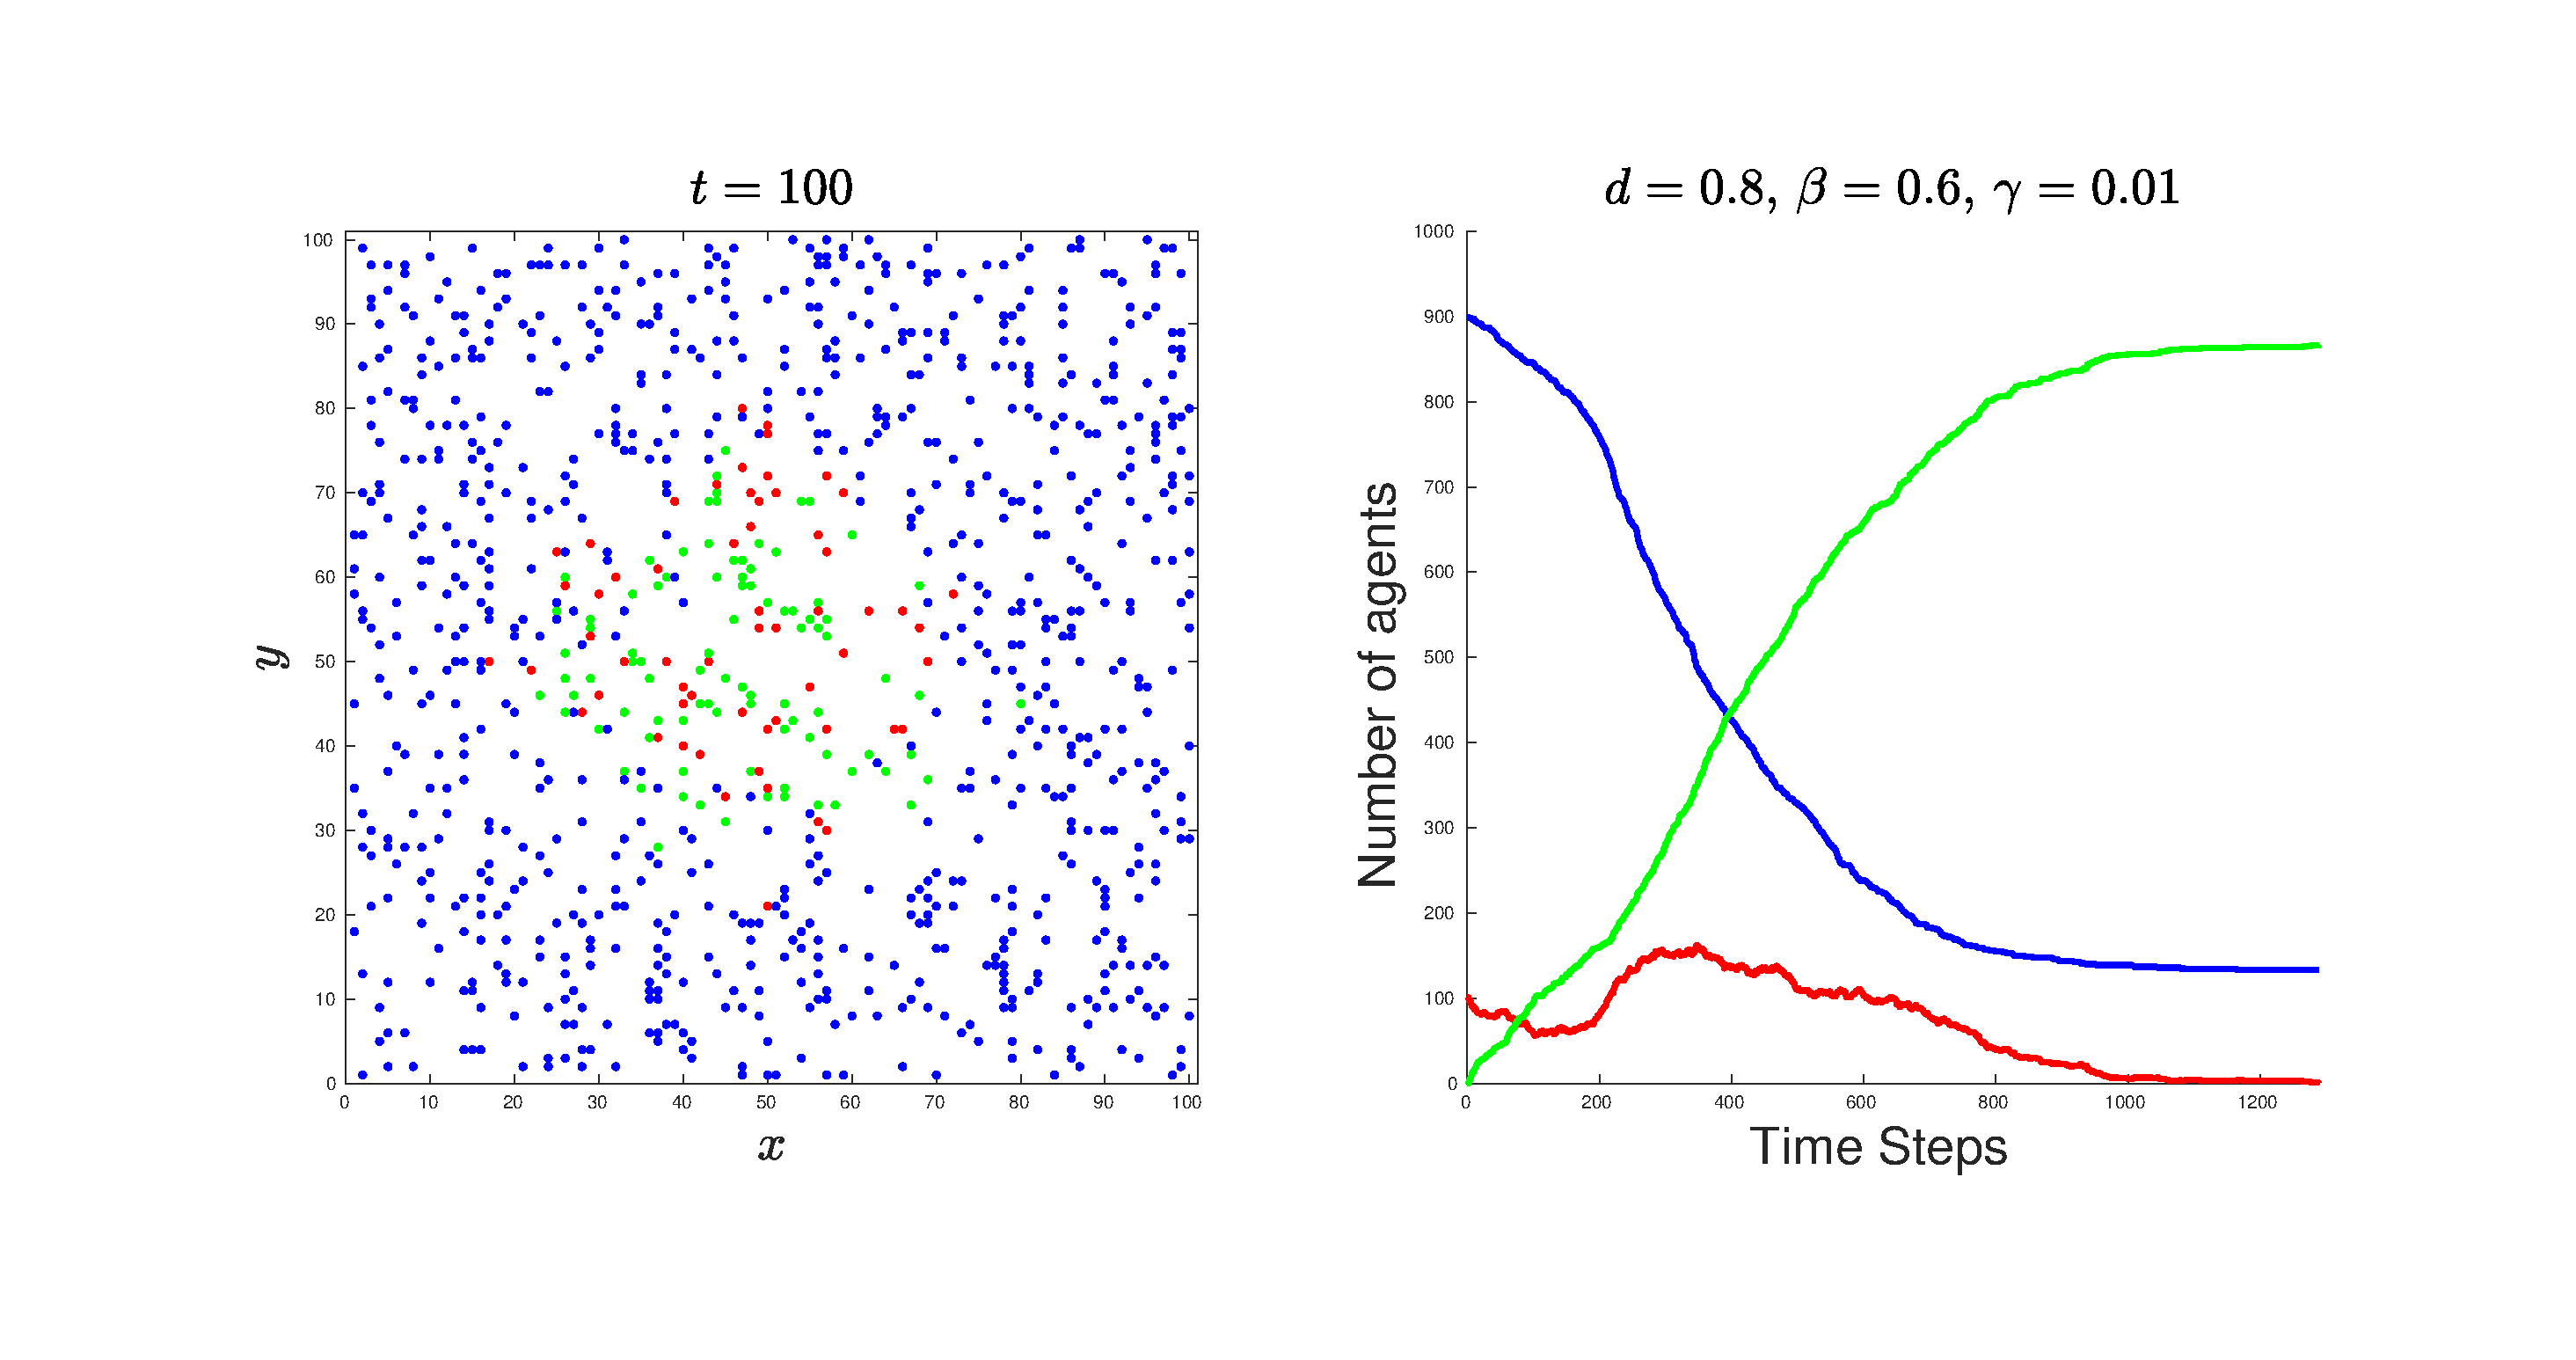
\includegraphics[width=0.9\linewidth]{1_1000_agents}
    \caption{Plot of the proportions of susceptible (blue), infected (red) and recovered (green) individuals in each state over time.}%
    \label{fig:2}
\end{figure}

With the above stated parameters ($d=0.8$, $\beta=0.6$, $\gamma=0.01$), the disease does not spread over the whole population. However over 80\% were infected over time, which could be a very likely scenario of the corona out brake.

\input{probabilistic_health_prediction.tex}

% !TeX root = ./main.tex
% chktex-file 46
% !TeX spellcheck = en-GB
% !TeX encoding = utf8

% - re-model current strategies: doing nothing, social distancing, isolation.

In the following we will present two extensions to the above methods.
First we demonstrate a baysian approach to estimate the populations' health state.
Second we show how the above methods could be utilized to derive disease containment policies.

\subsection{Baysian way of estimating the Probabilities}

A major drawback of our analysis is that we only take fixed disease states of individuals into account, i.e either susceptible, infected or recovered. However, in real live, due to the lack of data, these states are mostly unknown and have to be estimated by probability distributions. If we model these probabilities based on detailed assumptions, we can use Bayes' posterior probability to update these distributions based on the individual interaction of people. Thus, we define $X$ as the random variable that represents the state of a single individual. It can be assumed, that $X$ is well approximated by the multinomial distribution ($n\gg1$):
\begin{equation}
    X = \left(X_{S}, X_{I}, X_{R}\right) \sim \text{Mn}(n;p_S^{(t)},p_I^{(t)},p_R^{(t)})
\end{equation}
where $n$ is the population size, and $p_S^{(t)}$, $p_I^{(t)}$, and $p_R^{(t)}$ are the probability for an individual to be either in susceptible, an infected or recovered state. These probabilities change over time as the disease progresses, while

\begin{equation}
    p_S^{(t)}+p_I^{(t)}+p_R^{(t)}=1.
\end{equation}

As we can only estimate the probabilities $p_S^{(t)}$, $p_I^{(t)}$, and $p_R^{(t)}$ from samples of our population with a certain error, we assume that the probabilities are realisations of a prior distribution, in this case the Dirichlet distribution:

\begin{equation}
    \left(p_{S,i}^{(t)}, p_{I,i}^{(t)}, p_{R,i}^{(t)}\right) \sim \operatorname{Dir}\left(\alpha_{S,i}^{(t)}, \alpha_{I,i}^{(t)}, \alpha_{R,i}^{(t)}\right).
\end{equation}

The pseudo-counts $\alpha_{1,i}^{(0)}$, $\alpha_{2,i}^{(0)}$, and $\alpha_{3,i}^{(0)}$ can be estimated from $p_S^{(0)}$, $p_I^{(0)}$, and $p_R^{(0)}$ and are equal for each individual $i$ at $t=0$. Because we have no additional prior information, we also choose $\sum_{i\in\{S,I,R\}}\alpha_i = 1$.

If we now assume that two individuals with unknown state meet at the same location, an interaction occurs and we cannot neglect, that at least one of the individuals may carry the disease and may potentially infect the other. Therefore, we assume, that each individual is present in an infectious superstate $\braket{x}$ where
\begin{equation}
    \braket{x} = \left(\braket{x_{S,i}}, \braket{x_{I,i}}, \braket{x_{R,i}}\right) = \left(p_S^{(t)},p_I^{(t)},p_R^{(t)}\right)
\end{equation}
If the state of an individual in this group known, due to a previous test for example, the state collapses into the right state (e.g $(0,1,0)$ for an infected individual).

Based on this either known or super positional state, we can define the graph based Bayesian update rule of the pseudo-counts, where the infection rate $\beta$ is also taken into account, as followed~\cite{rice2006mathematical}:

\begin{align}
    \alpha_{S,i}^{(t+1)\prime} &= \alpha_{1,i}^{(t)\prime}\\
    \alpha_{I,i}^{(t+1)\prime} &= \alpha_{2,i}^{(t)\prime} + \beta \cdot
    \sum_{j\in A^{(t)}_{v_i}} A^{(t)}_{i,j} x_{I,j}\\
    \alpha_{R,i}^{(t+1)\prime} &= \alpha_{3,i}^{(t)\prime}\\
    \alpha_{0,i}^{(t+1)\prime} &= \alpha_{S,i}^{(t+1)\prime}+\alpha_{I,i}^{(t+1)\prime}+\alpha_{R,i}^{(t+1)\prime}
\end{align}

Important to notice is that the adjacent $A$ has to be normalized to $\operatorname{max}(A)=1$, where $A_{v_i,v_j}=1$ means a direct contact between individual $v_i$ and individual $v_j$.
In this step, the update is only done for the $\alpha_I$, as only the possible infection of an individual can change the infection state of another individual.

However, so far this model still does not take the potential recovery into account. We can add this by looking at the estimated Values of $p_{S,i}^{(t+1)}$, $p_{I,i}^{(t+1)}$, and $p_{R,i}^{(t+1)}$ 
\begin{alignat}{2}
    \operatorname{E}[p_{S,i}^{(t+1)}] &= \frac{\alpha_{S,i}^{(t+1)\prime}}{\alpha_{0,i}^{(t+1)\prime}} & &= \frac{\alpha_{S,i}^{(t+1)}}{\alpha_{0,i}^{(t+1)\prime}} \\
    \operatorname{E}[p_{I,i}^{(t+1)}]&= \frac{\alpha_{I,i}^{(t+1)\prime}}{\alpha_{0,i}^{(t+1)\prime}}-\gamma & &=\frac{\alpha_{I,i}^{(t+1)}}{\alpha_{0,i}^{(t+1)}} \\
    \operatorname{E}[p_{R,i}^{(t+1)}]&= \frac{\alpha_{R,i}^{(t+1)\prime}}{\alpha_{0,i}^{(t+1)\prime}}+\gamma & &= \frac{\alpha_{R,i}^{(t+1)}}{\alpha_{0,i}^{(t+1)}}
\end{alignat}

Based on this equation system, we can calculate $\alpha_{k,i}^{(t+1)}$ for $k\in{S,I,R}$. Needless to say, that if the expectation value of $p_{I,i}^{(t+1)}$ or $p_{R,i}^{(t+1)}$ return a value smaller than 0 or larger than 1, we set $\gamma=0$ and therefore $\alpha_{k,i}^{(t+1)\prime}=\alpha_{k,i}^{(t+1)}$. Something similar may be found in~\cite{stojanovic2019bayesian}.

We see here, that the probability for an individual to be in the susceptible state shrinks over time, the more contacts with people have been observed. Thus, if we set this individual into quarantine, the probabilities shift towards either the susceptible state or the recovered state. This is an early indicator, why it is necessary to put the whole population under quarantine in the case of a pandemic.

We can now find an optimal test setup by applying tests to those individuals, who's unknown infection state introduce the most uncertainty to our estimation. Furthermore, we could even set individuals with a high probability to have the disease under quarantine, without testing them (which should be an urgent object of an ethical discussion).



\subsection{Policy Design}
In the previous sections we have shown how predict the health state of all individuals in a location tracked population.
The next step is to use this information to compute optimal policies.
These policies guide a governments' and societies' response to the spread of COVID-19 and modify how the disease is able to spread in a population.

An optimal policy always keeps the infection counts below the medical systems' capacity and the total number of infections as small as possible.
% not much real data on this.
Mathematically speaking we want to minimize the sum of all future infections
\begin{equation}\label{eq:number-of-infected}
	\min \sum_{\forall t} N^{(t)}_i
\end{equation}
whilst
\begin{equation}\label{eq:cap-constraint}
	N^{(l)}_i \leq N_{limit}, \forall t
\end{equation}

A policy may consist out of two different kinds of actions, non pharmaceutical interventions (NPI) and test prioritization (TP).


\subsubsection{Non Pharmaceutical Interventions (NPI)}
All non pharmaceutical interventions can be understood as some kind of edge removal in our graph-based approach:
\begin{itemize}
	\item Isolation of an infected individual removes all of its edges with very high probability.
	\item Quarantine of a contact person removes all of its edges with high probability.
	\item Social distancing removes some edges of many individuals.
	\item Cancellation of large events remove many edges of many individuals.
\end{itemize}

Formally speaking, the square matrix $C \in \mathbb{B}$ with dimensions $N \times N$ models desirable edge cancellations.
This is the policy, which will be optimized.
To avoid the trivial solution of $C=0$, the cancellation of all edges, we also want to minimize the the number of cancellations
\begin{equation}\label{eq:cancellations}
	\min_{C} -\sum_i \sum_j C_{ij}
\end{equation}

Note, that this matrix does not have to know the edges of a future time step, it only expresses which edges must not exist.
It is multiplied element-wise onto the adjacency matrix $A$ to obtain the adjacency matrix with applied cancellations $\bar{A} = A \odot C$.

% Future Work: This would be more powerful, if there would be some different kinds of edges (social, work, education, large events, etc.)\\
% Future Work: This only takes the current time step into account but it would be desirable to look even further into the future.

To obtain an optimal cancellation policy one thus must jointly minimize \cref{eq:number-of-infected,eq:cancellations} whilst fulfilling \cref{eq:cap-constraint}.

\subsubsection{Test Prioritization (TP)}
When tests are limited, we argue that they should be used to discover as much as possible about the health state of the overall population.
This in turn allows non pharmaceutical interventions such as school cancellations to become more efficient.
Currently there are only rough medical-based guidelines who should be tested and who should not.

Lets assume there are $t_{\text{max}}$ tests per time step.
A test reveals the true health state of an individual (ignoring false negatives and false positives)
\begin{equation}
h_{{v}_i}^{(t)} \xrightarrow{\text{test}} h_{{v}_i}^{(t+1)} \in \{\vec{e}_0, \vec{e}_1, \vec{e}_2 \}
\end{equation}

The test assignment $T$ with dimension $N$ is a binary variable describing which individuals should be tested.

% !TeX root = ./main.tex
% chktex-file 46
% !TeX spellcheck = en-GB
% !TeX encoding = utf8

\section{Consistency of notations}%
\label{sec:consistency}

Using the notation from the blog and the paper, including $H'\in\mathbb{R}^{N\times D}$, $A\in\mathbb{R}^{N\times N}$, $H\in\mathbb{R}^{N\times D}$, the propagation rule is:

\begin{equation}
	H' = A H
\end{equation}

is equivalent to

\begin{equation}
	\begin{split}
		H'_{v_i, m} & = \sum_l \overbrace{A_{v_i, l}}^{\in \{0, 1\}} H_{l, m} \\
		            & = \sum_{l'} H_{l',m}
	\end{split}
\end{equation}

where $l'$ takes all $A_{v_i,l}=1$, i.e.\ neighbours, into account.

Hence, I do understand that the notations are equal.

\section{Formulate normalisation}

Use from ICLR 2017 paper the normalisation $D_{ii} = \sum_j \hat{A}_{ij}$.

Use the knowledge from the blog post to write:

\begin{equation}
	\begin{split}
		\overbrace{H'}^{\in \mathbb{R}^{N\times D}} & = \overbrace{D^{-1}}^{\in\mathbb{R}^{N\times N}} \overbrace{\hat{A}}^{\in \mathbb{R}^{N\times N}} \overbrace{H}^{\in\mathbb{R}^{N\times D}} \\
		\Leftrightarrow H'_{v_i, m} & = \sum_k \overbrace{D^{-1}_{v_i,k}}^{=D_{v_i,v_i}, \delta_{v_i, k}} {(\hat{A} H)}_{km} \\
			& = D^{-1}_{v_i, v_i} {(\hat{A} H)}_{v_i, m} \\
			& = D^{-1}_{{v}_i, v_i} \sum_k \hat{A}_{v_i, k} H_{k, m} \\
			& = \sum_k \underbrace{\frac{\hat{A}_{v_i, k}}{\sum_j \hat{A}_{v_i, j}}}_{\text{normalised}} H_{k, m}.
	\end{split}
\end{equation}

The weighting by the adjacency matrix is, indeed, normalised to its column sums.

Note that this part is also normalised:

\begin{equation}
\begin{split}
	\sum_m H'_{v_i, m} & = \sum_m \sum_k \frac{\hat{A}_{v_i, k}}{\sum_j \hat{A}_{v_i, j}} H_{k, m} \\
	& = \sum_k \frac{\hat{A}_{v_i, k}}{\sum_j \hat{A}_{v_i, j}} \underbrace{\sum_m H_{k,m}}_{=1\text{, per construction}} \\
	& = 1
\end{split}
\end{equation}

\newpage
\raggedright{}
\bibliography{bibliography}


\printbibliography{}

\end{document}
